% Created 2022-02-23 Wed 11:06
% Intended LaTeX compiler: pdflatex
\documentclass[11pt]{article}
\usepackage[utf8]{inputenc}
\usepackage[T1]{fontenc}
\usepackage[margin=3cm,a4paper]{geometry}
\usepackage{graphicx}
\usepackage{grffile}
\usepackage{longtable}
\usepackage{subcaption}
%\usepackage{wrapfig}
%\usepackage{rotating}
%\usepackage[normalem]{ulem}
\usepackage{amsmath}
%\usepackage{textcomp}
\usepackage{amssymb}
%\usepackage{capt-of}
\usepackage{hyperref}
\author{Mridul Gupta}
\date{Monday 21 February 2022 IST}
\title{ELL888 Minor}
\hypersetup{
 pdfauthor={Mridul Gupta},
 pdftitle={ELL888 Minor},
 pdfkeywords={},
 pdfsubject={},
 pdfcreator={Emacs 27.1 (Org mode 9.3)}, 
 pdflang={English}}
\begin{document}

\maketitle
\section{Q1}
\label{sec:orge586eff}
This problem has a straight forward approach. First generate the
missing data and then use the data matrix as if it was a normal matrix
to learn graph structure.\par The data generation process itself,
however, is non-trivial. And the exact method used depends a lot on
the data being used as well as the mechanics of data being
missing. Since in this case the data is missing at random, one can
completely ignore the missing data and just use complete
features~\cite{links_1}.\par
Note that this only works when the fraction of data missing is not
huge. For example if \(70-80\%\) of data is missing, then we cannot
ignore all the data. However, in such cases the best remedy is to
collect more data properly.\par
Now, imputing new data can be done in several ways. One method is to
just replace the missing data points with a default value. A little
improvement over this is calculating the mean (or median) for each
feature and replacing missing value in a feature with it its mean.\par
The mean uses the distribution information, and we can go one step
further by learning the distribution/density on the features and
sample random variables from the distribution. This works for iid
samples and iid features.\par
This requires assumption of the form of distribution of the
features. One popular missing data generating method is the
EM-algorithm. The recursive EM-algorithm is more popularly used with
the assumption that the density is a mixture of Gaussians.\par
Another method can be to use can be to learn \(d\) regression models,
each for a feature. The \(k^{\text{th}}\) model uses features
\(\{i\}_{i\neq k}\) to predict the value of feature \(k\). This method
will inherently incorporate dependencies between features as well as
the learn the density of the feature we are predicting. One problem
might be some other feature \(j\neq k\) might also have missing value;
a solution to this is to use mean (or median) as the placeholder of
feature \(j\) during prediction of feature \(k\).
\subsection{Experimentation}
\label{sec:org8003e69}
For this problem, I work with two datasets: seeds~\cite{repo,seeds} (from
\href{https://archive.ics.uci.edu/ml/datasets/seeds}{here}) and wine~\cite{repo,wine} (from \href{https://www.kaggle.com/harrywang/wine-dataset-for-clustering}{here}). Both of these are complete
datasets with real valued features. Seeds dataset has 7 real valued
features. The wine clustering dataset has 11 real valued and 2 integer
valued features but I just drop them.\par
Since we need missing data, I randomly delete \(1\%\) of values within
the dataset. I then create \(k\) GaussianMixture models trained using
Expectation Maximization algorithm to learn densities of the \(k\)
features. I then use the learned means and covariances to sample a
random value to be used as an estimate of given feature. Graph is
learned using the imputed feature matrix.
\begin{figure}[!htbp]
\centering
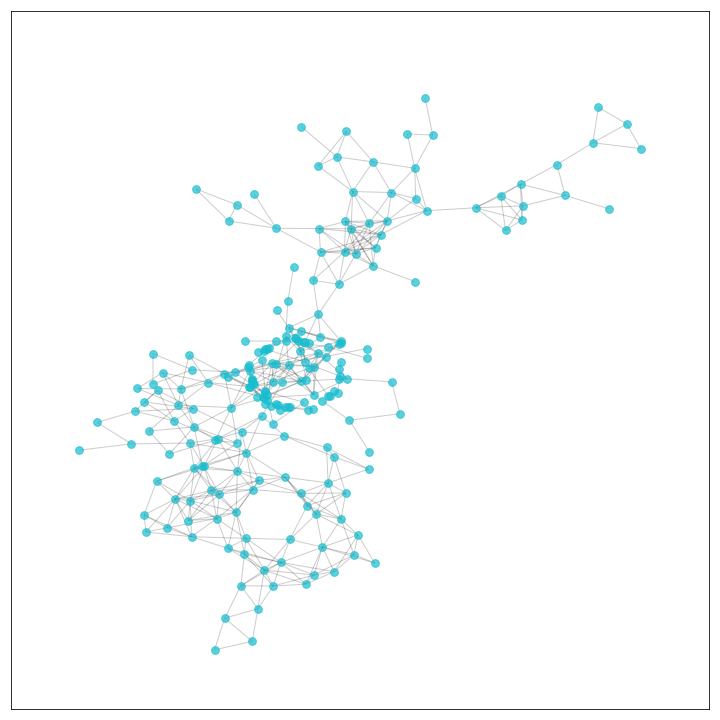
\includegraphics[width=.9\linewidth]{/home/mridul/Desktop/exam/ELL888/code/sSeeds.png}
\caption{Graph learned on Seeds dataset}
\end{figure}
\begin{figure}[!htbp]
\centering
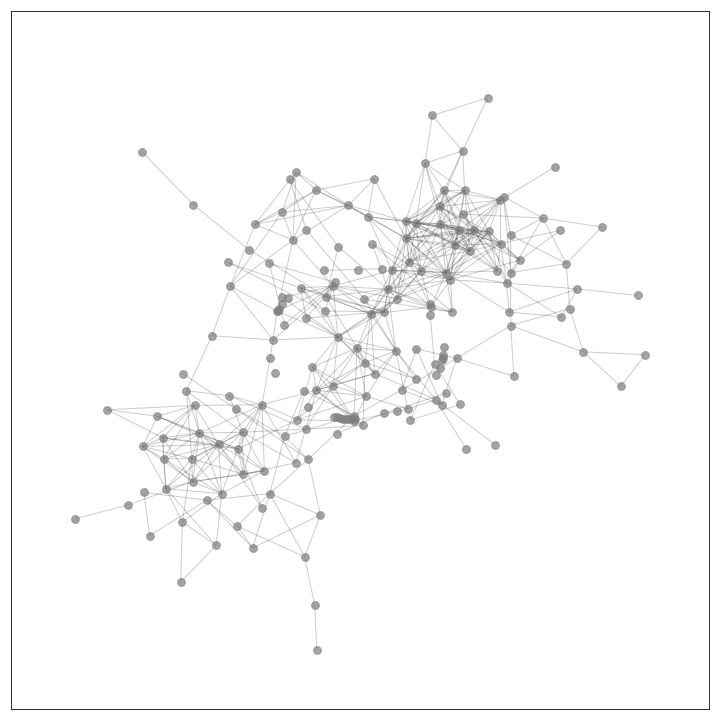
\includegraphics[width=.9\linewidth]{/home/mridul/Desktop/exam/ELL888/code/sWine.png}
\caption{Graph learned on Wine clustering dataset}
\end{figure}
\clearpage
I also try with larger missing value percentages \((10\%)\), and perform
missing value imputation using \(k\)-regression models. Calculating the Euclidean distance
between generated versus original data in both kinds of imputation reveals reduction in
distance by almost a factor of \(\frac{1}{2}\). Here are the graphs generated in the two settings:
\begin{figure}[!htbp]
    \begin{center}
        \subfloat[EM-Algorithm]{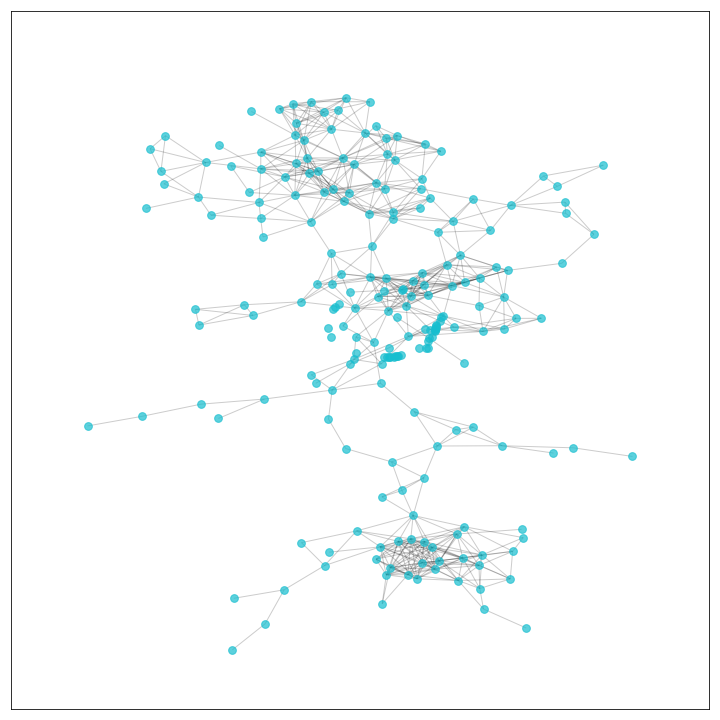
\includegraphics[width=0.5\linewidth]{/home/mridul/Desktop/exam/ELL888/code/sSeeds2.png}}
        \subfloat[Regression]{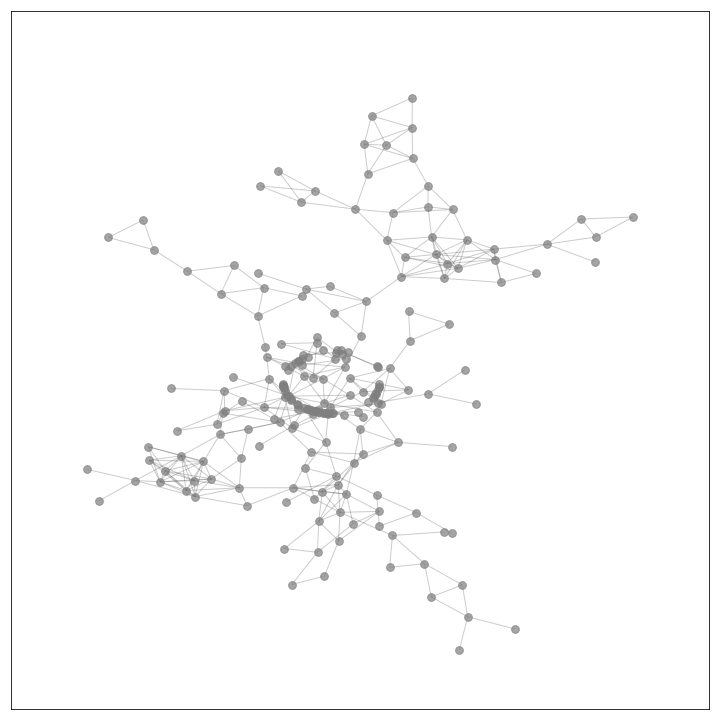
\includegraphics[width=0.5\linewidth]{/home/mridul/Desktop/exam/ELL888/code/sRegression.png}}
        \caption{Seeds dataset}
    \end{center}
\end{figure}
\begin{figure}[!htbp]
    \begin{center}
        \subfloat[EM-Algorithm]{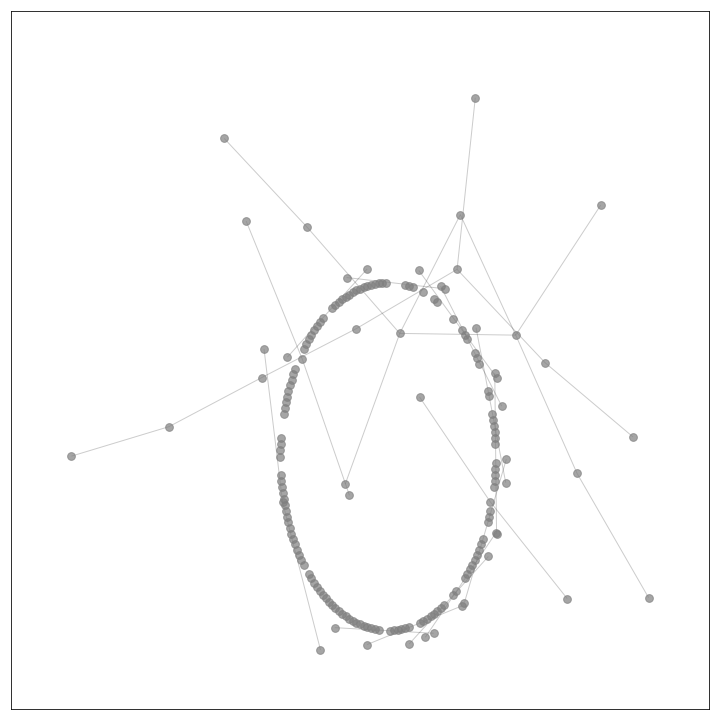
\includegraphics[width=0.5\linewidth]{/home/mridul/Desktop/exam/ELL888/code/sWine2.png}}
        \subfloat[Regression]{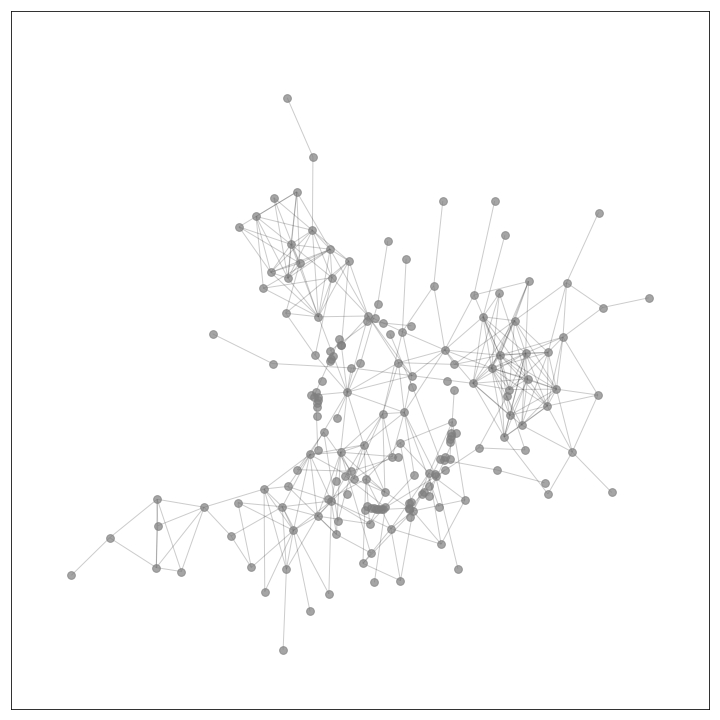
\includegraphics[width=0.5\linewidth]{/home/mridul/Desktop/exam/ELL888/code/RegressionWine.png}}
        \caption{Wine clustering dataset}
    \end{center}
\end{figure}
\clearpage
\section{Q2}
\label{sec:org1cffea9}
Since \(y_i\in\{0,1\}\), a solution that incorporates label
information is as follows:\\
Choose a distance metric \(D(x_1,x_2)\). Update distance metric to
be \(\tilde{D}(x_1,x_2)=D(x_1,x_2)+k(1\{y_1=1-y_2\}-1\{y_1=y_2\})\) if
both \(y_1\text{ and }y_2\) are available, else just use \(D(x_1,
x_2)\) without the label information. Calculate second order
statistics matrix and learn graph.\par
So, taking this approach, for experimentation I chose MNIST
handwritten digits dataset~\cite{MNIST}.\par
The MNIST dataset is really big for the purposes
\(\text{(}\mathbf{X}\in\mathbb{R}^{60000\times 784}\text{)}\) of this
question, so I select \([10,50,100,500]\) images and project this
smaller subset using PCA onto \(\mathbb{R}^15\). Also, since the
question uses the assumption of \(y\in\left\{0,1\right\}\), I make
this selection such that all images are of class 0 or 1 (MNIST has 10
classes from 0 to 9).\par
Next, I randomly choose \(40\%\) of the labels to be ignored. And just
construct the graph from the data (figure~\ref{fig:1}). I also learn a graph
without using label information (figure~\ref{fig:2}).
\begin{figure}[!h]
\centering
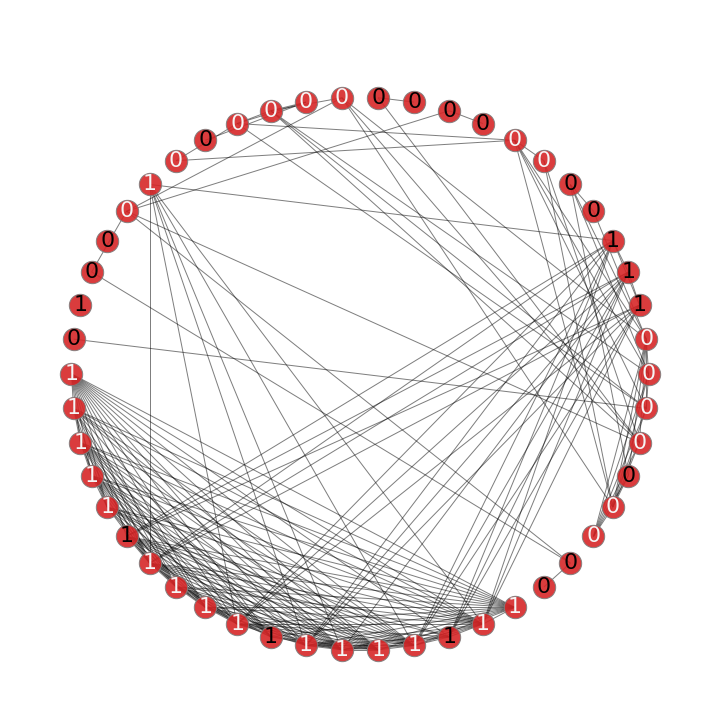
\includegraphics[width=.9\linewidth]{/home/mridul/Desktop/exam/ELL888/code/svGenerated_graph_50.png}
\caption{Graph with partially seen labels (white labels are observed, black are unobserved)}
    \label{fig:1}
\end{figure}
\begin{figure}[!h]
\centering
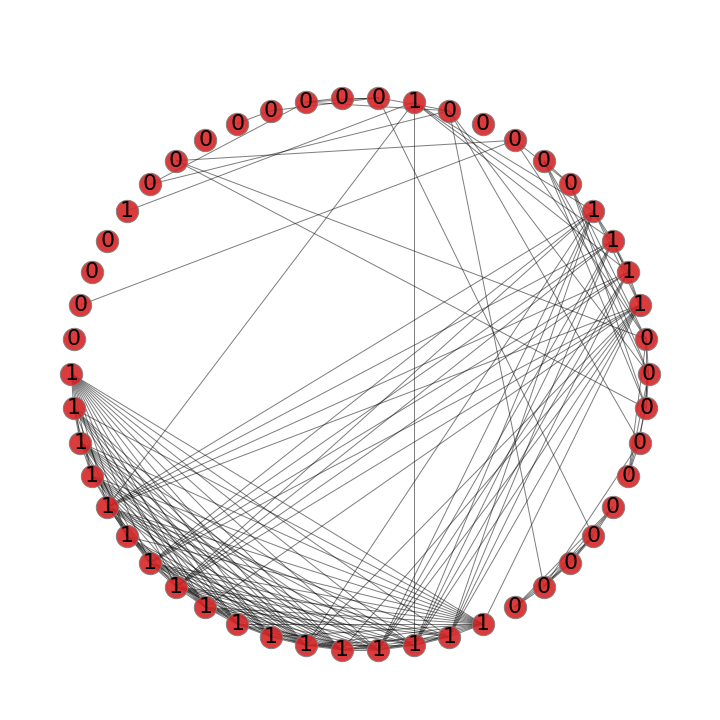
\includegraphics[width=.9\linewidth]{/home/mridul/Desktop/exam/ELL888/code/svGenerated_graph_without_info_50.png}
\caption{Graph with no seen labels}
    \label{fig:2}
\end{figure}
One thing to notice is that even though the graph structure isn't much
different in the latter case there are two 0's connected to a 1 as
seen in figure~\ref{fig:3}.
\begin{figure}[!h]
\centering
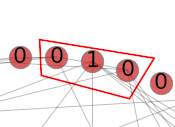
\includegraphics[width=.9\linewidth]{/home/mridul/Desktop/exam/ELL888/code/close_up.png}
\caption{Graph with no seen labels}
    \label{fig:3}
\end{figure}
so it can be said that the label information is being used, even if to
a small extent.
\clearpage
\section{Q3}
\label{sec:org3f21d58}
In this problem we have the data matrix \(X\in\mathbb{R}^{n\times d}\)
where both \(n\) and \(d\) are large, typically with \(n\gg d\). The
problem here is in calculating the second order statistics matrix. The
computation cost will be of the order \(O(n^2d)\). Since we need a
final adjacency and/or a weight matrix \(\in\mathbb{R}^{n\times n}\)
we cannot avoid the \(n^2\) in the cost term, but we can try to reduce
the \(d\) component.\par
Another problem is of fitting the big data matrix in memory to perform
computations. For really large matrices, they need to be stored in
hard drive which makes the computation difficult, unless one has
access to powerful compute resources.
\subsection{Developing the idea}
\label{sec:org4836409}
One of the key things that makes what follows work is the assumption
(which would generally be true) that the data is quite sparse. This
means we can compress the information to a lower dimensional
space.\par
Now, there are several ways to go about this. One way could be to do
PCA (or SVD) on the data \(X\in\mathbb{R}^{n\times d}\) to get
\(X^{PCA}\in\mathbb{R}^{n\times k}\) for some \(\mathbb{Z}^+\ni k \ll
d\). This new data can then be used to learn the graph. The
computation complexity of PCA is \(O(\min(d^3,n^3)\) which is
\(O(d^3)\) in our case. And with the second order statistics
calculation the complexity becomes \(O(d^3+n^2k)\).\par
Another problem remains however: the closed form PCA algorithm makes use of the
full data matrix, which might not fit into the memory for really large
\(n\text{ and }d\).
\subsection{Better solution (?)}
\label{sec:orga81f2dd}
As mentioned in the hint, it would be good if we could use stochastic
gradient descent based approaches. And the straight forward solution
is to use the extension of PCA that makes use of stochastic gradient
descent: a deep learning architecture called \textbf{AutoEncoder}.\par
An AutoEncoder consists of two neural networks: an \textit{encoder}
and a \textit{decoder}.
\begin{center}
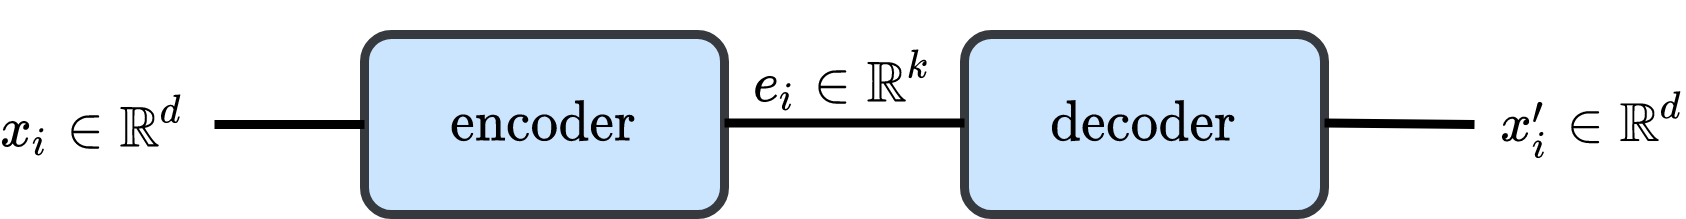
\includegraphics[width=.9\linewidth]{/home/mridul/Desktop/exam/ELL888/autoencoder.png}
\end{center}
The encoder takes in the data item \(x_i\in\mathbb{R}^d\) and outputs
an encoded embedding \(e_i\in\mathbb{R}^k\) while the decoder takes
this embedding and tries to reproduce the data from this compressed
representation. This can then be trained end-to-end using stochastic gradient
descent in minibatched fashion with mean squared error loss calculated
on \(x\text{ and }x'\). The idea is that if the embedding is useful
and retains information, then original data should be reproducible
given the embeddings.\par
Once the training is completed, the decoder is discarded and just the
encoder is used to generate embeddings from data. And once we have
this, we can learn the weight matrix using a kernel that looks at
pairs of data points at a time. For example a Gaussian Kernel can be
used as shown in equation~\ref{eqn:gaus}.
\begin{equation}
w_{ij}=\operatorname{exp}\biggl[-\frac{d(e_i,e_j)}{2\sigma^2}\biggr]
\label{eqn:gaus}
\end{equation}
Note: an autoencoder without non-linearities learns the same
embeddings as PCA.
\subsection{Advantages}
\label{sec:orgb58fa9b}
\begin{itemize}
\item Easily parallelizable.
\item Reduces data dimension that mitigates ``curse of dimensionality''.
\item Works on part of data that can be loaded into memory from hard drive
in advance by efficient data loader making it faster after the first
few data loads.
\item Can be trained on part of the data. It is generally required to have
more data than the number of parameters to avoid overfitting. Using
a validation set to keep a check on the generalization error
provides further improvement.
\end{itemize}
\subsection{Disadvantages and challenges}
\label{sec:org0a859e6}
\begin{itemize}
\item Fine tuning the parameter \(k\) is a challenge.
\item Since this works like a look up (that is take a data point and
generate its embedding), this can only be used with methods that
generate \(w_{ij}\) by looking only at \(x_i\) and
\(x_j\). Algorithms that use something like k-nearest neighbor
information are still a challenge.
\end{itemize}
\subsection{Experimentation}
\label{sec:org74c0d6b}
I use the MNIST handwritten digit dataset~\cite{MNIST} for this
task. This consists of \(60000\) images, each of size \(28\times 28\), so
the data matrix \(\mathbf{X}\in\mathbb{R}^{60000\times 28\times 28}\)
or equivalently \(\mathbf{X}\in\mathbb{R}^{60000\times 784}\) after
converting the image matrices into vectors. This data is still small,
but it'll work for this purpose.\par
I choose two projection size \(15\text{ and }5\) and test on
both. Note this is a lot of compression and it is expected a lot of
information will be lost.\par
The \(60000\) sized dataset is still too large for my machine, and the
naive but unavoidable \(\displaystyle\frac{n(n-1)}{2}\) calculations take a lot of
time so I chose a still smaller subset of size \(3000\) to do my
weight matrix calculations. The only way to go beyond this is to
parallelize these calculations using GPU.
\begin{figure}[!htbp]
\centering
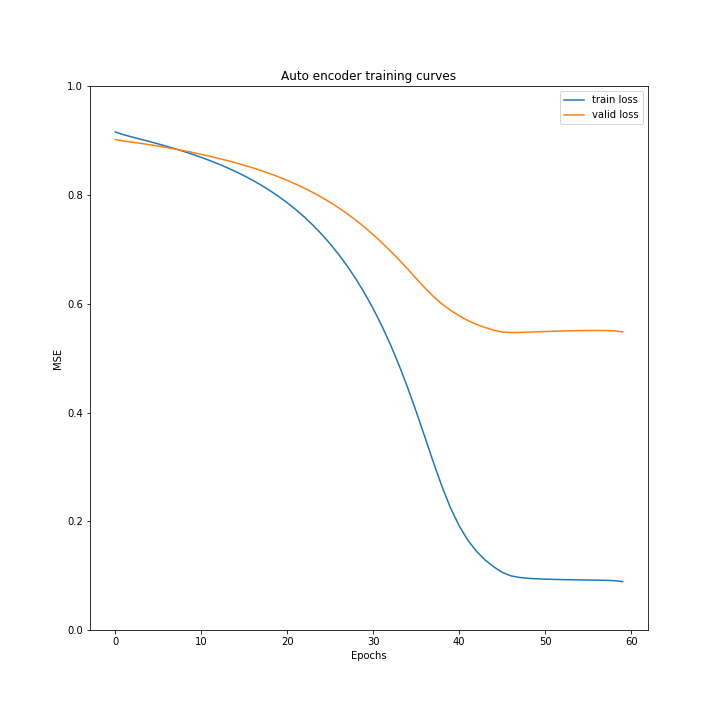
\includegraphics[width=.9\linewidth]{/home/mridul/Desktop/exam/ELL888/code/sAutoencoder_training_curves.png}
\caption{Projection size 15}
\end{figure}
\begin{figure}[!htbp]
\centering
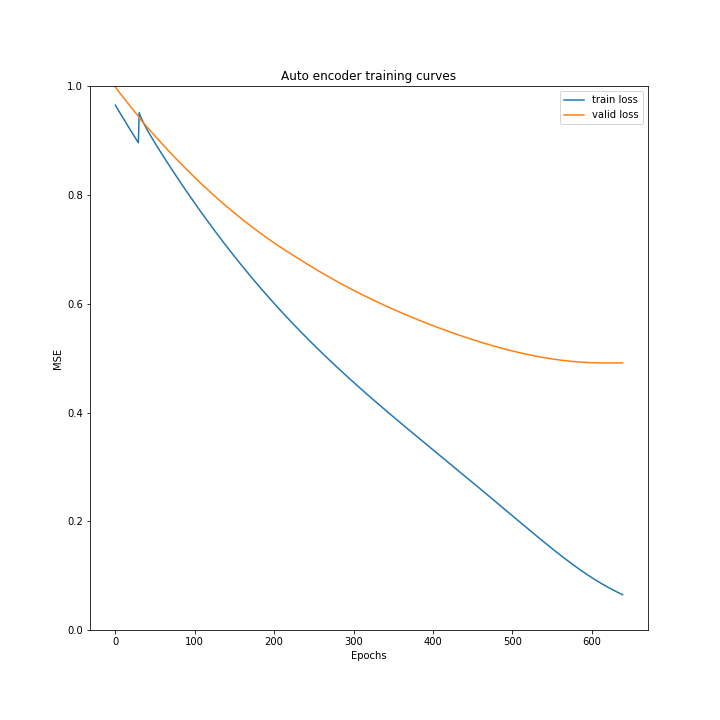
\includegraphics[width=.9\linewidth]{/home/mridul/Desktop/exam/ELL888/code/ssAutoencoder_training_curves.png}
\caption{Projection size 5}
\end{figure}
\clearpage
\section{Q4}
\label{sec:orga751ec2}
The problem with hetergeneous data can be solved by embedding the data
points into a real vector using something similar to the previous
question. Another much simpler approach is to simply define a distance
function that works with heterogeneous data to generate the second
order statistics matrix.\par
\subsection{Approach}
\label{sec:org1c60d9b}
The assumption here is that unlike the previous question, the data is
not of high volume, but that the challenge is that graph learning
frameworks usually work with numerical data.\par
So, we need a function that can calculate the elements of the second
order statistics matrix. And this can be done by defining a distance
function for various different kinds of data. Say we partion
\(\mathbf{X}\in\mathbb{R}^{n\times d_r}\times \mathbb{I}^{n\times d_i}
\times\mathbb{C}^{n\times d_c}\) as
\([\mathbf{X_R},\mathbf{X_I},\mathbf{X_C}]\). Then we can define a
suitable distance function on each of the partition.\par
For example, say we use the Euclidean distance (equation~\ref{eqn:eucl}) on both real and
integer partitions.
\begin{equation}
D_{\text{eucl}}(x^i,x^j) = \biggl(\sum_{k=1}^{d_{\text{partition}}}(x^i_k-x^j_k)^2\biggr)^{\frac{1}{2}}
\label{eqn:eucl}
\end{equation}
And use the Hamming distance after one-hot encoding the categorical
data (equation~\ref{eqn:hamm}).
\begin{equation}
D_{\text{hamm}}(x^i,x^j)=\sum_{k=1}^{d_c} x^i\oplus x^j
\label{eqn:hamm}
\end{equation}
With these two, the final distance can then be defined as a weighted
sum as shown in equation~\ref{eqn:dist}.
\begin{align*}
N(x^i, x^j)=&W_r\cdot D_{\text{eucl}}(x^i_{1:d_r},x^j_{1:d_r})\\
&+W_i\cdot _{\text{eucl}}(x^i_{d_r:d_r+d_i},x^j_{d_r:d_r+d_i})\\
&+W_c\cdot D_{\text{hamm}}(x^i_{d_r+d_i:d_r+d_i+d_c},x^j_{d_r+d_i:d_r+d_i+d_c})\\
\end{align*}
\begin{equation}
D(x^i,x^j)=\frac{N(x^i,x^j)}{W_r+W_i+W_c}
\label{eqn:dist}
\end{equation}
\subsection{Next steps}
\label{sec:org34c02f3}
Once we have the second order matrix weights can be generated from it
using kernel methods, linear embeddings, nearest neighbor methods,
laplacian based methods for structural constraints, etc.
\subsection{Advantages}
\label{sec:org2f30ab2}
\begin{itemize}
\item Works with heterogeneous data
\item Little modification required in anything else
\end{itemize}
\subsection{Disadvantages}
\label{sec:org12d5ffa}
\begin{itemize}
\item Works when data is small. If data is large however, then one must
consider embedding to lower dimension similar to previous question
since autoencoders can also be used with categorical (after one-hot
encoding) and integer data.
\end{itemize}
\subsection{Other possible approaches}
\label{sec:orgd49153f}
One can also consider using other data structures such as trees (and
metrics they use, like gini index or mutual information) since they
work well with heterogeneous data.
\subsection{Experimentation}
\label{sec:org5cc286a}
The dataset selected was hepatitis dataset~\cite{repo,hep,hep2} found \href{https://archive.ics.uci.edu/ml/datasets/Hepatitis}{here}. It
has 20 features, 14 of which were categorical, 4 integers and 2 are
real valued. Using the above method, the following graph was generated
\begin{center}
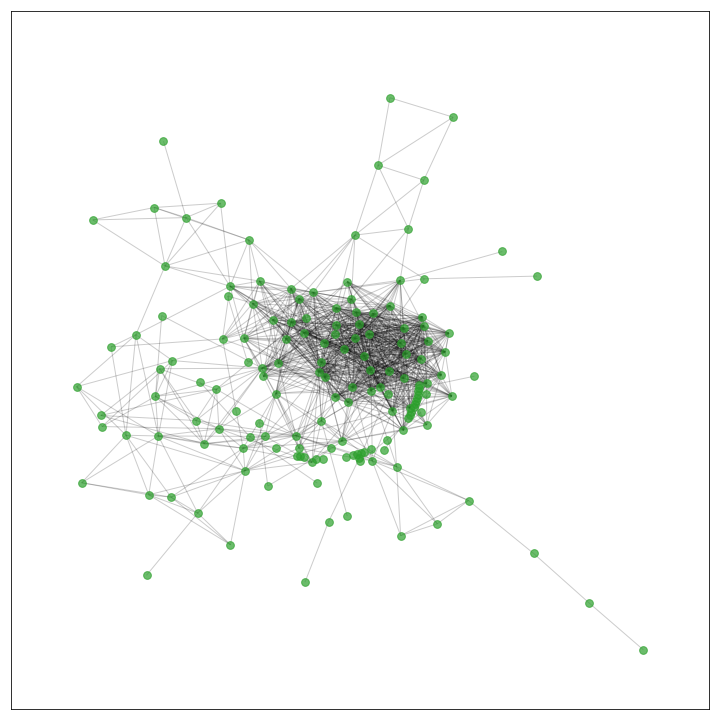
\includegraphics[width=.9\linewidth]{/home/mridul/Desktop/exam/ELL888/code/shepatitis.png}
\end{center}
\bibliographystyle{ieeetr}
\bibliography{ref.bib}
\end{document}
